\documentclass[11pt, a4paper, twoside]{article}

% Version en 2024 Víctor Bettachini < vbettachini@unlam.edu.ar >

\usepackage[T1]{fontenc}
\usepackage[utf8]{inputenc}

% \usepackage[spanish, es-tabla]{babel}
% \def\spanishoptions{argentina} % Was macht dass?
% \usepackage{babelbib}
% \selectbiblanguage{spanish}
% \addto\shorthandsspanish{\spanishdeactivate{~<>}}

\usepackage{graphicx}
\graphicspath{{../figuresLaTeX/}}
% \usepackage{float}

\usepackage[arrowdel]{physics}
\newcommand{\pvec}[1]{\vec{#1}\mkern2mu\vphantom{#1}}
% \usepackage{units}
\usepackage[separate-uncertainty= true, multi-part-units= single, range-units= single, range-phrase= {~a~}, locale= FR]{siunitx}
\usepackage{isotope} % $\isotope[A][Z]{X}\to\isotope[A-4][Z-2]{Y}+\isotope[4][2]{\alpha}

\usepackage{tasks}
\usepackage[inline]{enumitem}
% \usepackage{enumerate}

\usepackage{hyperref}

% \usepackage{amsmath}
% \usepackage{amstext}
% \usepackage{amssymb}

\usepackage{tikz}
\usepackage{tikz-3dplot}
\usepackage{tikz-dimline}
\usetikzlibrary{calc}
% \usetikzlibrary{math}
\usetikzlibrary{arrows.meta}
\usetikzlibrary{snakes}
\usetikzlibrary{decorations}
\usetikzlibrary{decorations.pathmorphing}
\usetikzlibrary{patterns}

\usepackage[hmargin=1cm,vmargin=3cm, top= 0.75cm,nohead]{geometry}

\usepackage{lastpage}
\usepackage{fancyhdr}
\pagestyle{fancyplain}
\fancyhf{}
\setlength\headheight{28.7pt} 
\fancyhead[LE, LO]{\textbf{Computational Analytical Mechanics} }
% \fancyhead[LE, LO]{\textbf{Mecánica General} }
\fancyhead[RE, RO]{\href{https://ingenieria.unlam.edu.ar/}{$\vcenter{\hbox{\includegraphics[height=1cm]{ambos.pdf}}}$}}
\fancyfoot{\href{https://creativecommons.org/licenses/by-nc-sa/4.0/}{$\vcenter{\hbox{\includegraphics[height=0.4cm]{by-nc-sa_80x15.pdf}}}$} \href{https://ingenieria.unlam.edu.ar/}{DIIT - UNLaM}}
\fancyfoot[C]{ {\tiny Updated \today} }
\fancyfoot[RO, LE]{Page \thepage/\pageref{LastPage}}
\renewcommand{\headrulewidth}{0pt}
\renewcommand{\footrulewidth}{0pt}


\begin{document}
\begin{center}
  \textsc{\large Rigid Body | Continuous Mass Distributions}
\end{center}


\begin{enumerate}
	\item
	\textbf{Moment of Inertia Tensor of a Rod}\\
	A rod of mass \(m= \SI{1}{\kilo\gram}\)  and negligible cross-section compared to its length \(l= \SI{1}{\metre}\) is given.
	Align an axis (\(\hat{z}\)) with it. 
	\begin{tasks}(2)
		\task Calculate its moments of inertia.
		\task Show what happens with the products of inertia. 
	\end{tasks}


	\item
	\textbf{Convenient Axes for Calculating Moments of Inertia}\\
	Perspective views of various objects are drawn. On these, draw the axes intersecting at the most convenient point for calculating moments of inertia, that is, at the center of mass. Do the same with the two axes that correspond to the plane view projection.
	\vspace{-0.8cm}
	\begin{tasks}(4)
		\task 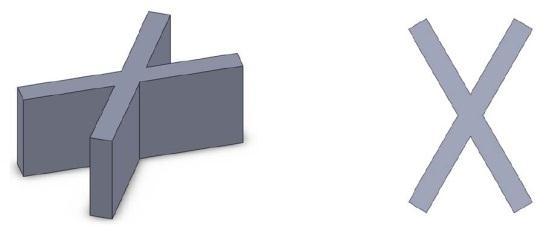
\includegraphics[width=0.15\textwidth]{figures/o-000}
		\task 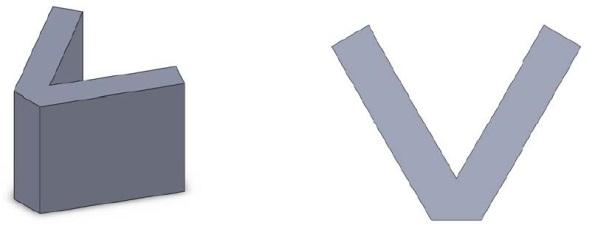
\includegraphics[width=0.15\textwidth]{figures/o-001}
		\task 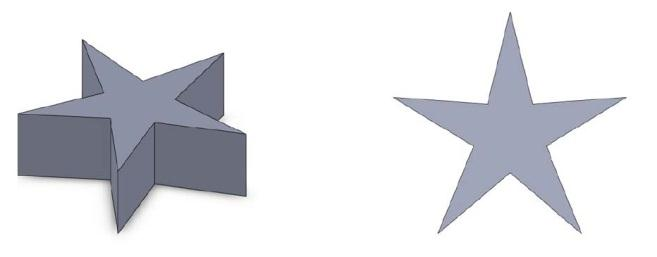
\includegraphics[width=0.15\textwidth]{figures/o-002}
		\task 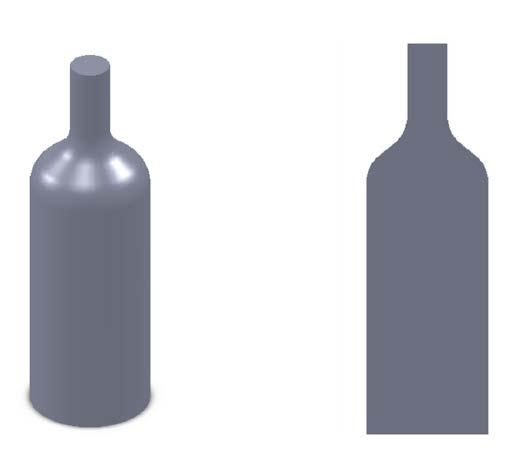
\includegraphics[width=0.15\textwidth]{figures/o-003}
	\end{tasks}


	\item 
	\begin{minipage}[t][4.5cm]{0.55\textwidth}
		% \begin{minipage}[t][3.5cm]{0.7\textwidth}
			\textbf{Cube with Edge \(b\)} [Marion (e) ex. 11-3]
			\begin{enumerate}
				\item Calculate the inertia tensor from the coordinate system \(x_i\) with origin at the center of mass \(O\).
				\item Use the general form of Steiner's parallel axis theorem to calculate it in the \(X_i\) system with origin at vertex \(Q\) 
			\end{enumerate}
		\end{minipage}
		\begin{minipage}[c][1cm][t]{0.4\textwidth}
			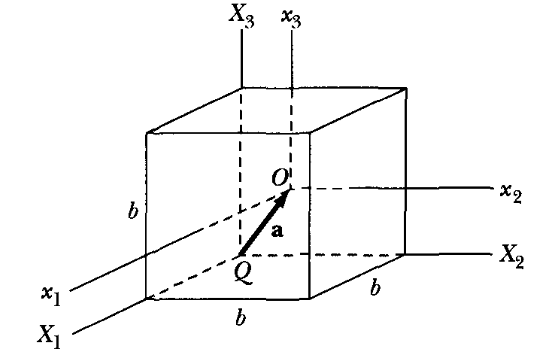
\includegraphics[width=\textwidth]{figures/mFig11-8}
		\end{minipage}


	\item 
		\begin{minipage}[t][4cm]{0.49\textwidth}
			\textbf{Perforated Plate}\\
			In a plate of homogeneous density, two openings were cut symmetrically. Suspended from point A, it \emph{oscillates} in the \(x,y\) plane. Therefore, it is relevant to know its moment of inertia \(I_{zz}\) from that point. Use the data available in a workshop: thickness $e$ of the material, plane dimensions, and a measured mass $m$. 

			Follow this suggested sequence:			
		\end{minipage}
		\begin{minipage}[c][2cm][t]{0.45\textwidth}
			\includegraphics[width=\textwidth]{figures/o-023}
		\end{minipage}
			\begin{enumerate}
				\item Calculate the metal density of the plate considering the missing area due to the perforations.
				\item Calculate \(I_{zz}\) of one of the circular perforations as if it were made of this metal.
				\item Calculate \(I_{zz}\) of an unperforated plate from its center of mass.
				\item Transfer with Steiner's theorem the \(I_{zz}\) of both circular perforations to the center of the plate.
				\item Subtract from the \(I_{zz}\) of the unperforated plate that of the circles to obtain that of the perforated plate.
				\item Again with Steiner's theorem, transfer the  \(I_{zz}\) of the perforated plate to pendulum point A.
			\end{enumerate}


			Result: 
			\(
			I_{zz} = \frac{m \left(- 12 \pi R^{4} - 6 \pi R^{2} a^{2} - 24 \pi R^{2} d^{2} + 4 a^{3} b + a b^{3}\right)}{12 \left(- 2 \pi R^{2} + a b\right)}
			\) 

	\item 
		\begin{minipage}[t][2.5cm]{0.62\textwidth}
			\textbf{Cylinder in Semi-cylinder} [Landau \S 32 6]\\
			Find the kinetic energy of a homogeneous cylinder of radius \(a\) rolling inside a cylindrical surface of radius \(R\).

			Result:
			\(
				T = \frac{3 m \left(R - a\right)^{2} \dot{\phi}^{2}}{4}
			\)
		\end{minipage}
		\begin{minipage}[c][1cm][t]{0.3\textwidth}
			\includegraphics[width=\textwidth]{figures/lFig41}
		\end{minipage}


	\item 
		\begin{minipage}[t][3.5cm]{0.72\textwidth}
			\textbf{Cone} [Landau \S 32 2e]\\
			This cone has a circular base of radius \(R\) and height \(h\).
			 \begin{enumerate}
				\item Calculate the position of the center of mass \(O\) from the vertex \(O'\).
				Remember to choose integration limits based on the geometry.
				Result: \(|\overline{O O'}| = \frac{3}{4} h\).
				\item Calculate the moments of inertia from \(O'\).\\
				Result: \(I_{x'_3 x'_3} = \frac{3}{10} m R^{2} \qquad I_{x'_1 x'_1} = I_{x'_2 x'_2} = \frac{3 m \left(R^{2} + 4 h^{2}\right)}{20}\)
			\end{enumerate}
			\end{minipage}
			\begin{minipage}[c][1cm][t]{0.2\textwidth}
			\includegraphics[width=\textwidth]{figures/landauFig38}
		\end{minipage}

	\newpage

	\item 
		\begin{minipage}[t][3.5cm]{0.53\textwidth}
			\textbf{Cone Rolling on a Plane} [Landau \S 32 7]\\
				 The instantaneous contact with the \(X Y\) plane, \(\overline{O A}\), forms angles \(\theta\) with \(X\) and \(\alpha\) with the cone's axis.
				 The other known datum is the distance to the center of mass \(a\).
				\begin{enumerate}
					\item Assuming known moments of inertia from the vertex in the axial direction \(I_3\) and in the perpendicular directions \(I_1 = I_2\), calculate the kinetic energy.
					Result:\\
					\(T = \frac{1}{2} \cos^2(\alpha) I_1 \dot{\theta}^{2} + \frac{1}{2} \frac{\cos^4(\alpha)}{\sin^2(\alpha)} I_3  \dot{\theta}^{2} + \frac{1}{2} \cos^2(\alpha) m a^{2} \dot{\theta}^{2} \)
					\item Express in the kinetic energy \(I_{1,2,3}\), \(\alpha\) and \(a\) as functions of the cone's base radius \(R\) and its height \(h\).
				\end{enumerate}
		\end{minipage}
		\begin{minipage}[c][0cm][t]{0.4\textwidth}
			\includegraphics[width=\textwidth]{figures/lFig42}
		\end{minipage}

\end{enumerate}

\end{document}
